% !TEX root =../main.tex

\chapter{Implementierung}

In diesem Kapitel wird dargestellt, wie ein Teil der Implementierung durchgeführt werden können. Angenommen, der Nutzer A will ein Computer in einem Webshop kaufen. Er besitzt nicht die Kenntnisse im Bereich von Hardware und Software um dies eigenständig zu tun. Eine Konfiguration vor Parametern fällt ihm Schwer. Er braucht die Hilfe von anderen Leuten.

\begin{description}
\item[Schritt 1:] Nutzer A loggt sich in den Webshop ein und sucht nach „Computer“.

\item[Schritt 2:] Viele unterschiedliche Computer erscheinen auf dem Bildschirm. Durch einen Vergleich des optischen Designs hat Nutzer A drei Marken ausgewählt. Er will durch drei Verkäufer bezüglich der drei ausgewählten Marken beraten werden. Des weiteren möchte er erfahren, welche Rabatte möglich sind.
\end{description}

Diese gewünschte Kommunikation könnte mittels PHP implementiert werden.

In Listing \vref{lst:php-chat} ist dargestellt, wie ein Online-Chat in PHP implementiert werden könnte.

\begin{lstlisting}[language=PHP, caption={Online-Chat in PHP}, label=lst:php-chat]
// socket-resource und die info vom Nutzer speichern

$connected_sockects = array(
  (int)$socket => array(
    'resource' => $socket,
    'name' => $name,
    'ip' => $ip,
    'port' => $port,
    ...
  )
);

// serverseite:TCP socket definieren

$this->master = socket_create(AF_INET, SOCK_STREAM, SQL_TCP);

// IP und port wiederverwendbar erstellen;
socket_set_option($this->master, SQL_SOCKET, SO_REUSEADDR, 1);
// IP und server werden mit socket verbunden;
socket_bind($this->master, $host, $port);
// mit listen funktion kann dieses socken von anderem socket angefragt werden;
socken_listen($this->master, self::LISTEN_SOCKET_NUM);

// der Server laufen
$write = $except = NULL

$sockets = array_column($this->sockets, 'resource'); // socket resource get
$read_num = socket_select($sockets, $write, $except, NULL);

foreach ($sockets as $socket) {
  if ($socket == $this->master) {
    socket_accept($this->master);
    // socket_accept() accept require" socket" verbinden;
    self::connect($client);
    continue;
  } else {
    // socket_recv() von socket die Laenge von len Daten ,in $buffer speichern
    $bytes = @socket_recv($socket, $buffer, 2048, 0);

    if ($bytes < 9) {
      // mit client unterbrochen
      $recv_msg = $this->disconnect($socket);
    } else {
      if (!$this->sockets[(int)$socket]['handshake']) {
        self::handshake($socket, $buffer);
        continue;
      } else {
        $recv_msg = self::parse($buffer);
      }
    }
    $this->broadcast($msg);
  }
}

// Infosform mit Json definieren
$msg = [
  'type' => $msg_type,
  'from' => $msg_resource,
  'content' => $msg_content, // info Inhalt
  'user_list' => $uname_list,
];
\end{lstlisting}

Auf seine Nachfrage erhält Nutzer A in 2 Sekunden eine Antwort bei Real-Time API. Zwei Verkäufer aus Dell und Acer versprechen, sie können einen attraktiven Rabatt anbieten.

\begin{description}
\item[Schritt 3:] Nutzer A entscheidet sich dafür, einen Computer von Dell oder Acer auszuwählen. Er will die Hardware und Komponenten vergleichen. Der Ehemann B von der Tochter seines Onkel‘s Cousin ist ein Hardwaretechniker. Nutzer A will die Hilfe von B bekommen.

\item[Schritt 3.1:] Die Kontakt Liste wird geöffnet, neue Kontaktperson hinzufügen. Der Telefonnummer von B wird eingegeben.

\item[Schritt 3.2:] \glqq{}Commit\grqq{} zu B gesendet. A ist glücklich. Wegen guter Freundschaft bestätigt B die Kontaktanfrage per SMS.
\end{description}

Die Verbindung zwischen Network und Mobile Smartphone:

Netzwerkstruktur

Im Gegensatz zu herkömmlichen Telekommunikationsdienstnetzwerken müssen wir nicht nur Server, sondern auch zentralisierte Server registrieren und Benutzerknoten in normale Knoten und Superknoten unterteilen. Registrierungsserver Systemverbindungsstruktur ist nachfolgend systematisch dargestellt.

\begin{figure}[htbp]
	\centering
	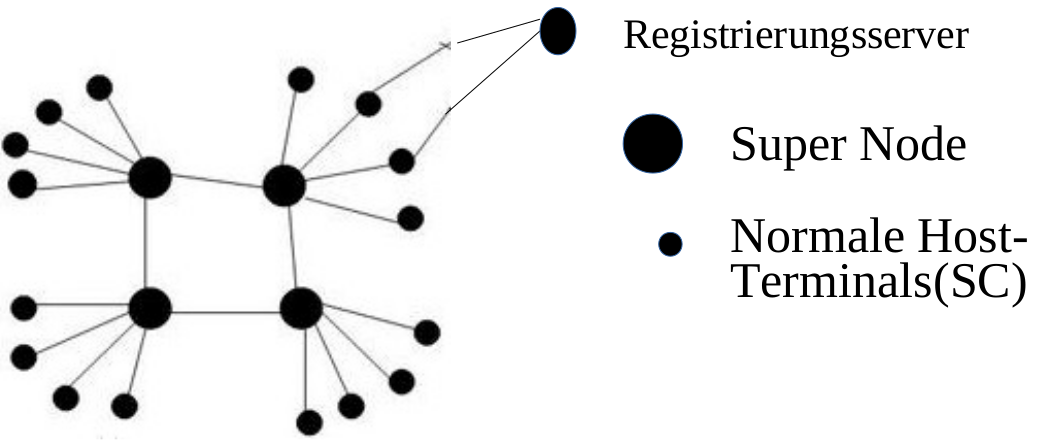
\includegraphics[width=0.4\textwidth]{bilder/telekommunikation-schema.png}
	\caption{Telekommunikation Schematisch}
	\label{fig:telekommunikation}
\end{figure}

Der Registrierungsserver ist ein Gerät, das gewartet werden muss. Es ist verantwortlich für das Registrieren des Clients, das Speichern und Verwalten von Benutzernamen und Kennwortinformationen. Wenn sich der Benutzer beim System anmeldet, wird der Benutzer authentifiziert. Der Registrierungsserver muss außerdem die globale Eindeutigkeit des Benutzernamens prüfen und garantieren.

Normale Knoten, d. h. normale Host-Terminals, müssen Online-Store-Anwendungen herunterladen, um Sprachanrufe und Textnachrichten bereitstellen zu können.

Der Supernode ist tatsächlich ein gewöhnlicher Knoten, der bestimmte Anforderungen erfüllt: Diese Anforderungen umfassen eine öffentliche Netzwerkadresse, eine ausreichende CPU, ausreichend Speicherplatz und eine ausreichende Netzwerkbandbreite. Mit anderen Worten, jedes geeignete Host-Terminal kann ein Super-Knoten werden, vorausgesetzt, die Anwendung wird geladen.


\section{Prozessmodell zur Beschreibung des Kaufprozesses}

\begin{figure}[htbp]
	\centering
	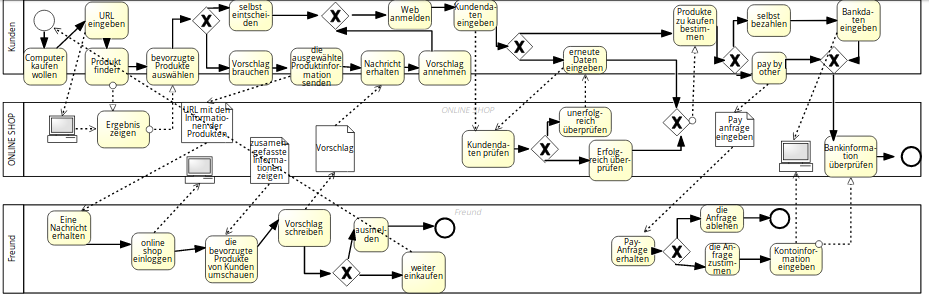
\includegraphics[width=1\textwidth]{bilder/bpmn-ablauf-kaufen.png}
	\caption{Ablauf des Kaufprozess}
	\label{fig:bpmn-ablauf-kaufen}
\end{figure}


\section{Freunde einladen}

\begin{figure}[htbp]
	\centering
	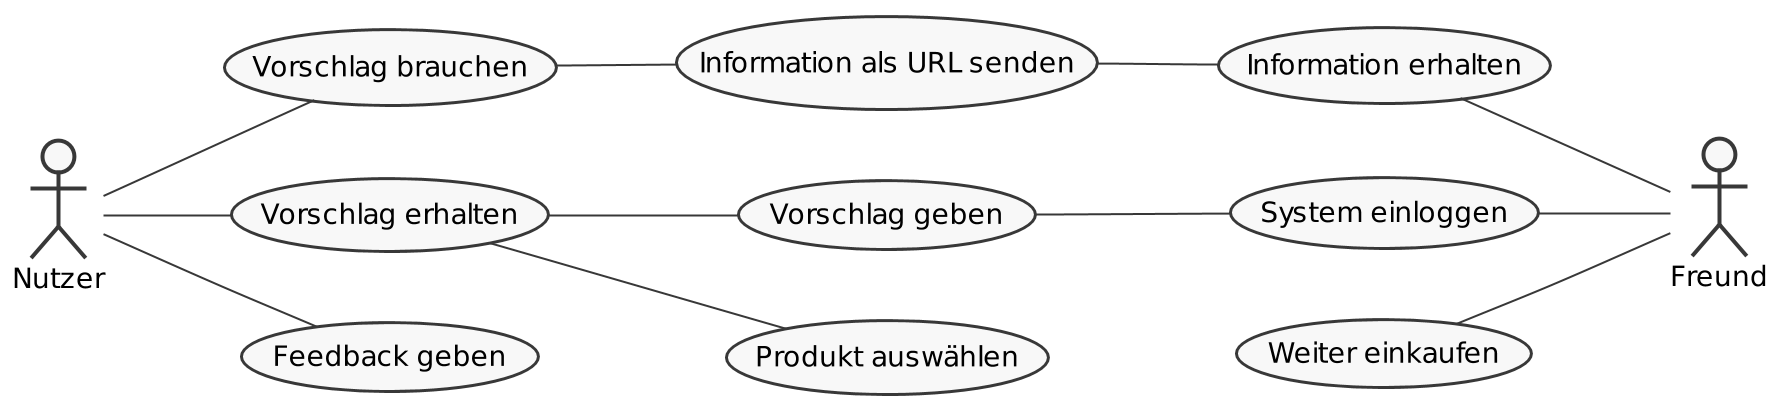
\includegraphics[width=1\textwidth]{uml-diagramme/freunde-einladen.png}
	\caption{Freunde einladen}
	\label{fig:freunde-einladen}
\end{figure}


\newpage

\section{Pay by Others}

\begin{figure}[htbp]
	\centering
	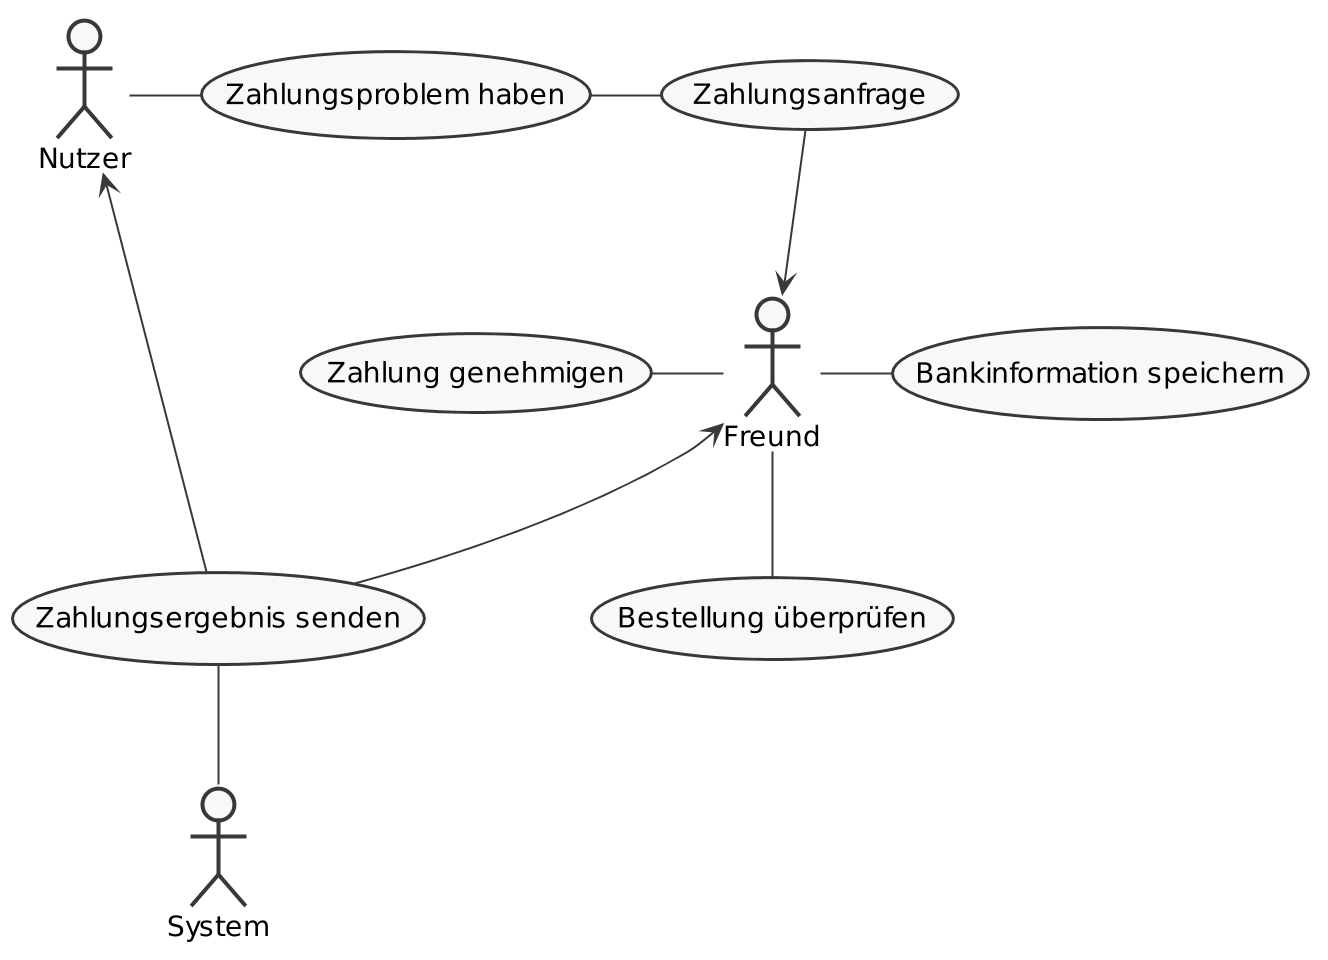
\includegraphics[width=0.8\textwidth]{uml-diagramme/pay-by-others.png}
	\caption{Pay by Others}
	\label{fig:pay-by-others}
\end{figure}


\section{Realtime Kommunikation}

\begin{figure}[htbp]
	\centering
	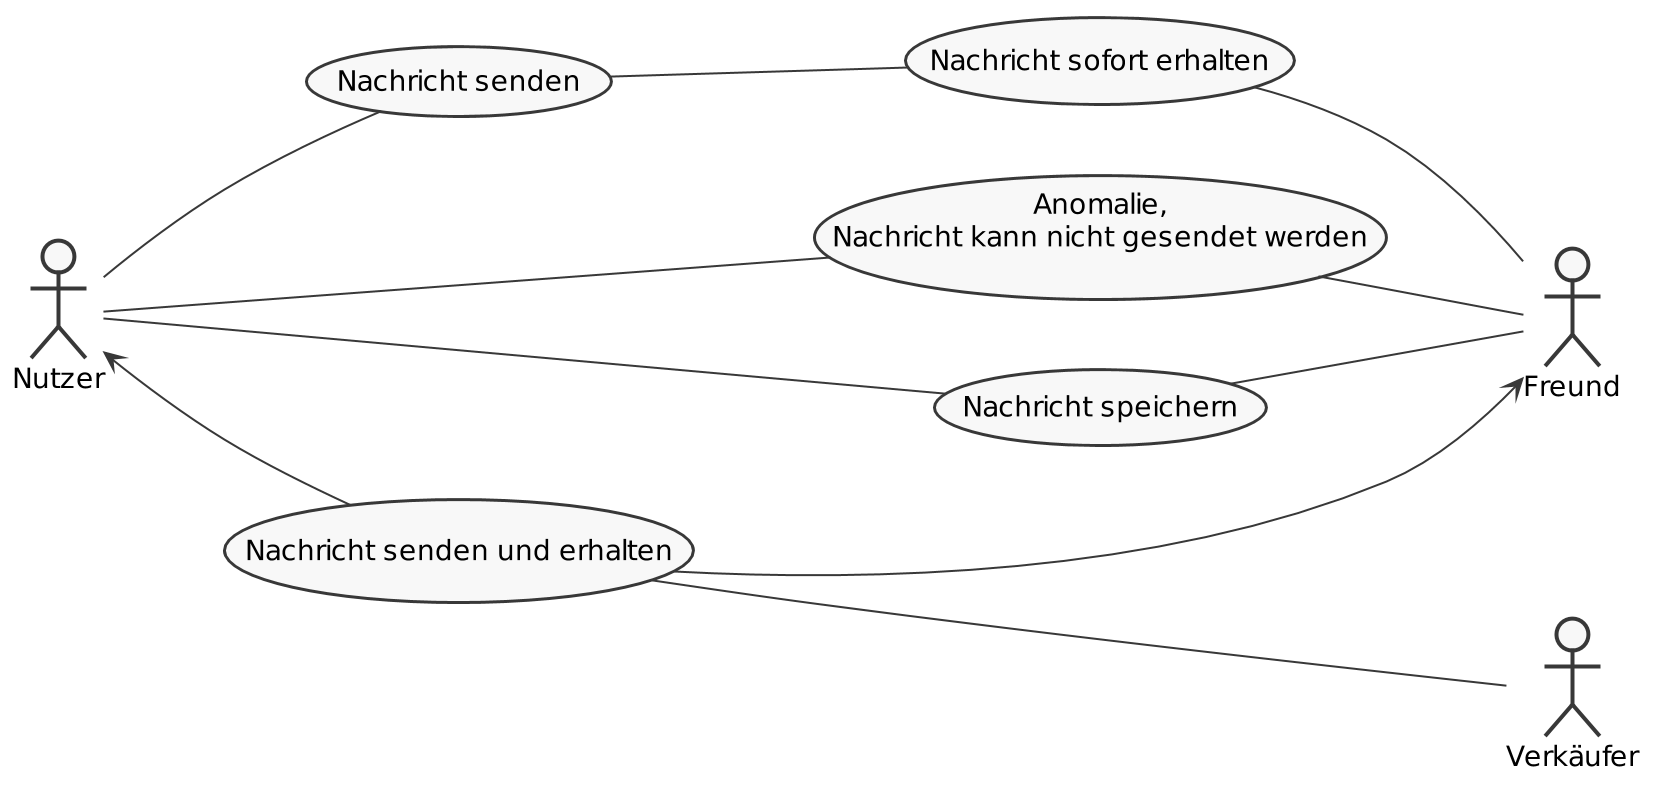
\includegraphics[width=0.8\textwidth]{uml-diagramme/real-time-communication.png}
	\caption{Realtime Kommunikation}
	\label{fig:real-time-communication}
\end{figure}
